\section{Modulo Utils}
\label{sec:moduloutils}

Questo terzo e ultimo modulo completa il pacchetto \texttt{GGH\_crypto}, offrendo algoritmi 
e strumenti generali e utili per i due crittosistemi descritti e implementati nelle sezioni 
precedenti. 
Anche in questo caso è caratterizzato da una classe \texttt{Utils} che,
sebbene priva di un costruttore, serve esclusivamente come contenitore per i metodi 
richiesti dai crittosistemi o per metodi indipendenti utili nella crittografia basata 
sui reticoli. Nelle prossime sottosezioni verranno esaminate e discusse le singole
funzioni, organizzate per categoria. 

\subsection{Conversione e norme}

La prima categoria di funzioni trattate riguarda quelle relative alla conversione e 
alle norme. Per quanto riguarda la conversione, sono presenti solo due funzioni specifiche:  
\texttt{npsp\_to\_fmpz\_mat} e \texttt{npsp\_to\_fmpq\_mat}, illustrate rispettivamente in 
Figura \ref{fig:npsp_to_fmpz_mat} e Figura \ref{fig:npsp_to_fmpq_mat}.
Come suggerisce il nome, queste funzioni eseguono la trasformazione di 
oggetti \texttt{Numpy} o \texttt{Sympy} in \texttt{fmpz\_mat} e \texttt{fmpq\_mat}. 
La conversione inversa non è necessaria, poiché \texttt{Numpy} e \texttt{Sympy} sono
in grado di interpretare 
istanze FLINT convertite in liste tramite il metodo \texttt{tolist} integrato in quest'ultimo.
Ulteriori conversioni non necessitano di funzioni proprie in quanto sono strettamente 
specifiche al contesto in cui si trovano. 
\begin{figure}[h]
    \begin{python}
        def sympy_to_fmpz_mat(basis):
            return fmpz_mat([[int(item) for item in sublist] 
                    for sublist in basis.tolist()])
    \end{python}
    \caption{Funzione di conversione da oggetti \texttt{Numpy} o \texttt{Sympy} a 
    \texttt{fmpz\_mat} contenuta nel modulo \texttt{Utils}.}
    \label{fig:npsp_to_fmpz_mat}
\end{figure}

\begin{figure}[h]
    \begin{python}
        def npsp_to_fmpq_mat(basis):
            fractions = [[Fraction(item) for item in row] 
                                    for row in basis.tolist()]
            return fmpq_mat([[fmpq(f.numerator, f.denominator) 
                                for f in row] for row in fractions])
    \end{python}
    \caption{Funzione di conversione da oggetti \texttt{Numpy} o \texttt{Sympy} a 
    \texttt{fmpq\_mat} contenuta nel modulo \texttt{Utils}.}
    \label{fig:npsp_to_fmpq_mat}
\end{figure}

Le norme contenute in \texttt{Utils} includono la L1 ed L2. La norma 
L2, implementata tramite la funzione \texttt{vector\_l2\_norm}, è osservabile 
in Figura \ref{fig:conversione} Sezione \ref{sec:FLINT}, 
mentre la norma L1 segue una struttura simile, differenziandosi principalmente per un 
calcolo leggermente più complesso, poiché le due norme misurano distanze in modi diversi.
Quest'ultima norma è implementata tramite la funzione \texttt{vector\_l1\_norm}. 
Entrambe fanno uso di conversioni da \texttt{fmpq\_flint} a \texttt{Decimal} con una 
precisione dei calcoli settata a 50. 

\subsection{Scrittura e lettura su file}

La seconda categoria di funzioni concerne quelle riguardanti la scrittura e la lettura,
su file di testo, di matrici FLINT.
Due sono le funzioni appartenenti a questa categoria:

\begin{itemize}
    \item \texttt{write\_matrix\_to\_file(matrix, filename)}: 
    Questa funzione consente di scrivere una matrice FLINT su un file di testo.
    Il parametro \texttt{matrix} rappresenta l'oggetto matrice da salvare, che può
    essere sia di tipo \texttt{fmpz\_mat} che \texttt{fmpq\_mat}. 
    Il parametro \texttt{filename} specifica il nome del file
    in cui salvare la matrice. La funzione costruisce automaticamente il percorso
    completo del file utilizzando la posizione dello script attualmente in esecuzione. Il contenuto
    della matrice viene scritto in un formato simile a una lista di liste Python,
    con ogni riga della matrice rappresentata come una lista interna. Gli elementi
    sono separati da spazi all'interno di ogni riga, e le righe sono separate dal
    carattere newline, ovvero \texttt{$\backslash$n}. Per le matrici \texttt{fmpq\_mat}, i
     numeri razionali
    vengono rappresentati nella loro forma frazionaria esatta.
    \item \texttt{load\_matrix\_from\_file(filename, matrix\_type='fmpq')}: 
    Questa funzione permette di leggere una qualsiasi matrice FLINT da un file di testo 
    precedentemente scritto con \texttt{write\_matrix\_to\_file}. 
    Il parametro \texttt{filename} specifica il percorso del file da cui leggere la matrice,
    mentre \texttt{matrix\_type} determina il tipo di matrice da caricare 
    ('fmpq' per matrici razionali o 'fmpz' per matrici intere, con 'fmpq' come valore 
    predefinito). La funzione
    gestisce automaticamente la conversione del contenuto del file nel formato appropriato,
    utilizzando il modulo \texttt{ast} per le matrici intere e un parsing personalizzato
    per preservare con precisione i valori razionali nelle matrici \texttt{fmpq\_mat}.
    Il parsing utilizza espressioni regolari con il modulo \texttt{re} per isolare le frazioni, 
    estraendo numeratore e denominatore. Questi valori vengono utilizzati per creare 
    oggetti \texttt{Fraction}, che vengono inseriti in una lista e successivamente convertiti 
    in una matrice \texttt{fmpq\_mat}, la quale viene infine restituita dalla funzione.

\end{itemize}
Anche se queste due funzioni non vengono impiegate direttamente dai crittosistemi, 
possono rivelarsi molto utili per il salvataggio di basi e vettori, facilitando così il 
loro riutilizzo in un secondo momento. Inoltre, entrambe sono utilizzate dal modulo 
\texttt{Utils} durante la fase di riduzione tramite BKZ usando FPLLL. Questo approccio è particolarmente 
vantaggioso perché la gestione dei dati tramite file rappresenta uno dei metodi più 
efficaci e affidabili, soprattutto nella comunicazione tra programmi in esecuzione su Windows e su
WSL. Utilizzare lo standard input e output potrebbe non essere 
sufficiente, considerata la grande quantità di dati e le elevate dimensioni coinvolte.

\subsection{Visualizzazione grafica}

\begin{figure}[h]
    \begin{python}
        from GGH_crypto import Utils
        from flint import fmpz_mat

        R = fmpz_mat([[1, 2],[3, 0]])
        B = fmpz_mat([[5, 4],[-6, -6]])
        T = fmpz_mat([[5, 3]])
        w1 = Utils.babai_rounding(R, V)

        w2 = Utils.babai_rounding(B, V)

        Utils.visualize_lattice(R, w1, T, B, w2, 
                        "Babai Visualization Example", limit=5)
    \end{python}
    \caption{Esempio di caso d'uso della funzione \texttt{visualize\_lattice}.}
    \label{fig:babaivisualizationcode}
\end{figure}

La terza categoria è relativa alla visualizzazione grafica dei dati grazie la libreria
\texttt{Matplotlib}, integrata nel modulo attraverso una funzione chiamata 
\texttt{visualize\_lattice}. I parametri in input accettabili dalla funzione sono:
\begin{itemize}
    \item \texttt{basis\_1} (\texttt{fmpz\_mat}): 
    Base dalla quale il reticolo viene generato e poi visualizzato, parametro solitamente
    usato per rappresentare la base privata. 
    \item \texttt{basis\_1\_cvp} (\texttt{fmpz\_mat}): 
    Vettore indicante il punto più vicino a un punto dato, ottenibile con gli algoritmi 
    dedicati usando il parametro \texttt{basis\_1}. 
    \item \texttt{point} (\texttt{fmpz\_mat})
    Vettore indicante un punto generalmente non appartenente al reticolo.
    \item \texttt{basis\_2} (\texttt{fmpz\_mat}, default: \texttt{None}): 
    Base secondaria anch'essa generante il reticolo, parametro solitamente
    usato per rappresentare la base pubblica. 
    \item \texttt{basis\_2\_cvp} (\texttt{fmpz\_mat}, default: \texttt{None}): 
    Vettore indicante il punto più vicino a un punto dato, ottenibile con gli algoritmi 
    dedicati usando il parametro \texttt{basis\_2}. 
    \item \texttt{title} (\texttt{String}, default: 'Lattice Plot'): 
    Stringa per impostare il titolo del grafico. 
    \item \texttt{limit} (\texttt{Integer}, default: 5): 
    Parametro intero per limitare la quantità di punti del reticolo nel grafico. 
\end{itemize}

Questa funzione è progettata per visualizzare un reticolo generato da una o due basi, 
insieme a punti di interesse specifici, generalmente pensata per la visualizzazione di dati
relativi al CVP. Per motivi di performance e complessità dell'output, le basi e i vettori 
passati come parametri devono avere una dimensione di massimo 2. 
La funzione inizialmente converte le basi e i vettori in array del modulo 
\texttt{Numpy}, in quanto, \texttt{Matplotlib} ci si interfaccia nativamente. 
Viene successivamente generata una griglia di coordinate intere (meshgrid) moltiplicata poi 
per \texttt{basis\_1}, dando origine quindi ai punti del reticolo.
La funzione visualizza il reticolo risultante, includendo con diversi colori
frecce per le basi, punti di interesse e annotazioni. Le dimensioni della visualizzazione 
vengono infine regolate automaticamente in base ai punti visualizzati. 

\begin{figure}[H]
    \centering
    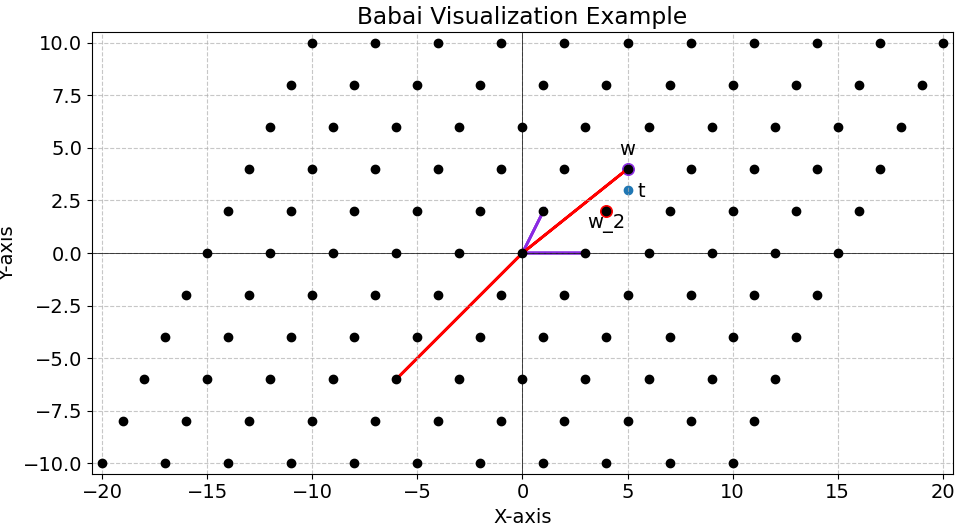
\includegraphics[width=\textwidth]{matplotlib.png}
    \caption{Esempio di visualizzazione della tecnica di arrotondamento di Babai con l'ausilio
    della funzione \texttt{visualize\_lattice}.}
    \label{fig:babaivisualizationout}
\end{figure}

Tale funzione è direttamente integrata negli algoritmi per la risoluzione del CVP
implementati in \texttt{Utils} e spiegati nella prossima selezione. 
E' possibile osservare un esempio d'uso in Figura \ref{fig:babaivisualizationcode} nel
quale sono stati usati i dati dell'Esempio \ref{exp:babai}. Il risultato è osservabile 
in Figura \ref{fig:babaivisualizationout}: in viola è rappresentata la base privata $\mathbf{R}$, 
insieme al risultato della tecnica di arrotondamento di Babai 
$\mathbf{w} \in \mathcal{L}(\mathbf{R})$ applicata a tale base.
In rosso sono illustrati la base pubblica $\mathbf{B}$ e il punto corrispondente 
$\mathbf{w\_2} \in \mathcal{L}(\mathbf{B})$ ottenuto utilizzando 
la stessa tecnica, ma con la base pubblica. In blu è invece 
evidenziato il punto $\mathbf{t} \notin \mathcal{L}(\mathbf{R})$, per il quale si richiede 
l'individuazione del punto più vicino appartenente al reticolo.


\subsection{Algoritmi di risoluzione del CVP}

La penultima categoria di funzioni si concentra sugli algoritmi per la risoluzione del 
CVP. Considerando le scelte di implementazione discusse nelle sezioni \ref{sec:moduloggh}
 e \ref{sec:moduloggh-hnf}, e seguendo la metodologia proposta da Nguyen nella crittoanalisi 
presentata in 
\cite{Nguyen99}, gli unici due algoritmi implementati nel modulo \texttt{Utils} 
sono la tecnica di arrotondamento di Babai e la tecnica di incorporamento. Il primo 
algoritmo, implementato attraverso la funzione \texttt{babai\_rounding},
è nettamente il meno complesso dei due in quanto si compone dei soli seguenti parametri:
\begin{itemize}
    \item \texttt{basis} (\texttt{fmpz\_mat}): Base con la quale l'algoritmo procederà 
    alla risoluzione del CVP. 
    \item \texttt{point} (\texttt{fmpz\_mat}): Punto non appartenente al reticolo generato 
    da \texttt{basis} con il quale l'algoritmo procederà alla risoluzione del CVP.
    \item \texttt{visualize} (\texttt{Boolean}, default: \texttt{False}):
    Se \texttt{True}, attiva la visualizzazione del reticolo chiamando la funzione 
    \texttt{visualize\_lattice} con i parametri \texttt{basis}, \texttt{point} e il CVP trovato.
\end{itemize}

\begin{figure}[h]
    \begin{python}
        def babai_rounding(basis, point, visualize=False):

            x = point * basis.inv()

            for i in range(x.nrows()):
                for j in range(x.ncols()):
                    x[i,j] = round(x[i,j])
            
            closest_vector = x * basis  

            if visualize:
                if basis.nrows() != 2:
                    raise ValueError("Dimension Error")
                Utils.visualize_lattice(basis, closest_vector, 
                    point, title="Babai rounding technique")
                
            return closest_vector
    \end{python}
    \caption{Implementazione della tecnica di arrotondamento di Babai contenuta nel modulo 
    \texttt{Utils}.}
    \label{fig:utilsbabai}
\end{figure}

L'implementazione mostrata in Figura \ref{fig:utilsbabai} è molto semplice, poichè
i passaggi da eseguire sono pochi e non richiedono una particolare complessità. 
Tutti i calcoli sono gestiti da FLINT, fatta eccezione per la funzione \texttt{round()},
integrata nativamente in Python.
Questa funzione viene direttamente chiamata da entrambe le implementazioni dei due 
crittosistemi, che poi gestiranno in maniera indipendente il risultato ritornato al
fine da ottenere il messaggio originale. 
Si può anche osservare che la visualizzazione grafica, gestita dal parametro visualize 
e realizzata tramite la funzione \texttt{visualize\_lattice}, viene eseguita solo dopo 
aver verificato che la base sia bidimensionale.
E' opportuno specificare che il controllo sul parametro \texttt{point} risulterebbe inutile
in quanto, se fosse di dimensione diversa dalla base, l'algoritmo ritornerebbe un errore 
a causa dell'impossibilità di moltiplicare matrici e basi di dimensioni diverse. 
La tenica di incorporamento invece, implementata attraverso la funzione \\
\texttt{embedding\_technique}, è sia teoricamente che implementativamente più complessa. 
Si compone dei seguenti parametri in input:
\begin{itemize}
    \item \texttt{basis} (\texttt{fmpz\_mat}):
    Base reticolare utilizzata nella fase di incorporamento.
    \item \texttt{ciphertext} (\texttt{fmpz\_mat}):
    Testo cifrato che verrà incorporato insieme alla matrice \texttt{basis} e al quale
    verrà sottratto il CVP ottenuto al termine dei calcoli.
    \item \texttt{visualize} (\texttt{Boolean}, default: \texttt{False})
    Flag booleana che, se impostata a \texttt{True}, inoltrerà \texttt{basis}, \texttt{ciphertext} e
    il CVP calcolato, alla funzione \texttt{visualize\_lattice} per ottenere un risultato
    grafico.
    \item \texttt{GGH} (\texttt{Boolean}, default: \texttt{False}):
    Flag che, se impostata a \texttt{True}, attiva una modalità specifica di ricerca del vettore più corto,
    considerando solo i vettori con l'ultimo elemento pari a 1.
    \item \texttt{BKZ} (\texttt{Boolean}, default: \texttt{False}):
    Se \texttt{True}, applica l'algoritmo BKZ invece di LLL per la riduzione del reticolo.
    \item \texttt{block} (\texttt{Integer}, default: 20):
    Dimensione del blocco da utilizzare nell'algoritmo BKZ, se attivato.
    \item \texttt{pruned} (\texttt{Boolean}, default: \texttt{False}):
    Se \texttt{True}, attiva la modalità di pruning nell'algoritmo BKZ. Questa modalità utilizza
    una strategia default per migliorare le performance dell'algoritmo 
    rinunciando però a parte della precisione nel calcolo della soluzione ottimale. 
    \item \texttt{precision} (\texttt{Integer}, default: 100):
    Precisione da utilizzare nei calcoli dell'algoritmo BKZ.
    \item \texttt{bkzautoabort} (\texttt{Boolean}, default: \texttt{True}):
    Se \texttt{True}, permette all'algoritmo BKZ di interrompersi automaticamente quando non si ottengono ulteriori miglioramenti.
    \item \texttt{bkzmaxloops} (\texttt{Boolean}, default: \texttt{False}):
    Se impostato a un valore intero, limita il numero massimo di iterazioni dell'algoritmo BKZ.
    \item \texttt{nolll} (\texttt{Boolean}, default: \texttt{False}): 
    Se \texttt{True} non verrà eseguita una riduzione LLL prima di procedere con la riduzione BKZ.
    La riduzione LLL non verrebbe effettuata da FLINT, ma bensì direttamente da FPLLL. 
\end{itemize}

L'implementazione di tale tecnica si compone inizialmente dalla costruzione della matrice
come descritto in Sezione \ref{sec:embedding} e mostrato nell'Esempoio \ref{exp:embedding}.
La costruzione fa uso unicamente di oggetti FLINT e list comprehension, metodi concisi
per la creazione di liste più o meno complesse in Python. A seconda del parametro \texttt{BKZ}
poi, viene deciso come effettuare la riduzione della matrice costruita: se tale parametro
è impostato a \texttt{True}, allora verrà fatta una chiamata alla funzione di riduzione BKZ presente in \texttt{Utils}
con il passaggio dei relativi parametri. In caso contrario l'opzione default è una riduzione
LLL tramite FLINT.  
Dopo la riduzione, l'algoritmo cerca il vettore più corto nella matrice ridotta. 
Il procedimento itera su tutte le righe, calcolando la norma L2 di ciascun vettore attraverso
la funzione integrata \texttt{vector\_l2\_norm} e tracciando quello con la norma minore.
Se il parametro \texttt{GGH} è \texttt{True}, il processo considera solo vettori con l'ultimo 
elemento uguale a 1, altrimenti considera tutti i vettori. 
Se l'algoritmo non trova vettori validi, viene eseguita una seconda ricerca 
considerando tutti i vettori disponibili. Questo approccio garantisce sempre la restituzione 
di un risultato, anche se potrebbe non essere la soluzione corretta al problema. 
Il CVP infine viene calcolato sottraendo il vettore trovato dal testo cifrato originale.
Anche questa funzione consente una visualizzazione grafica
del risultato attraverso il medesimo parametro \texttt{visualize} e gli stessi controlli 
implementati in \texttt{babai\_rounding}. 

\subsection{Riduzione e qualità di una base}



L'ultima categoria di funzioni presenti nel modulo \texttt{Utils} è quella relativa alla
misurazione della qualità di una base e alla sua riduzione. Per la prima tipologia è 
stata introdotta un'unica funzione, chiamata \texttt{get\_hadamard\_ratio},
responsabile del calcolo del rapporto di Hadamard, discusso
in Sezione \ref{sec:hadamard}. La sua implementazione, osservabile in Figura 
\ref{fig:utilshadamard}, si caratterizza dall'uso del modulo \texttt{Decimal} invece che
FLINT. Questa scelta è stata forzata dal fatto che FLINT non dispone nativamente dell'operazione
di elevazione alla potenza, che in questo caso deve essere fatta attraverso un numero frazionario.
Al fine di calcolare il determinante è stato comunque usato FLINT, mentre per il calcolo 
della norma è stata usata la funzione \texttt{vector\_l2\_norm}. 
La funzione \texttt{get\_hadamard\_ratio} accetta solo due parametri, ovvero:
\begin{itemize}
    \item \texttt{basis} (\texttt{fmpz\_mat} o \texttt{fmpq\_mat}): Base reticolare della
    quale viene calcolato il rapporto di Hadamard.
    \item \texttt{precision} (\texttt{Integer}, default: 10): Precisione con la quale 
    verranno effettuati i calcoli dal modulo \texttt{Decimal}. Questo parametro specifica
    inoltre di quante cifre decimali sarà composto il risultato formattato. 
\end{itemize}

\begin{figure}[H]
    \begin{python}
        def get_hadamard_ratio(basis=None, precision=10):
            norms = []
            dimension = matrix.nrows()
            
            getcontext().prec = precision
            
            for i in range(matrix.nrows()):
                row = fmpz_mat([[matrix[i, j] 
                                for j in range(matrix.ncols())]])
                norm = Utils.vector_l2_norm(row)
                norms.append(Decimal(str(norm)))
            
            log_denominator = sum(norm.ln() for norm in norms)
            log_numerator = abs(Decimal(matrix.det().str())).ln()
            
            log_result = (log_numerator - log_denominator) /
                                                Decimal(dimension)
            result = log_result.exp()
            
            return result, f"{result:.{precision}f}"
    \end{python}
    \caption{Funzione implementata nel modulo \texttt{Utils} e dedicata al calcolo del rapporto
    di Hadamard.}
    \label{fig:utilshadamard}
\end{figure}

Un aspetto rilevante dell'implementazione è l'ampio impiego di operazioni logaritmiche.
Operando nello spazio logaritmico, si prevengono problemi di stabilità numerica che 
potrebbero verificarsi manipolando direttamente numeri di scale molto diverse. Nel caso
del rapporto di Hadamard il problema può verificarsi nella produttoria di norme vettoriali,
che nel caso di matrici a grandi dimensioni, può causare un overflow. 
La funzione ritorna infine due valori: il risultato sottoforma di oggetto \texttt{Decimal}
e una sua versione formattata in stringa e limitata a \texttt{precision} cifre dopo la virgola. \\
La seconda tipologia, relativa alla riduzione di una base reticolare, è invece composta
dalle due funzioni \texttt{gram\_schmidt} e \texttt{BKZ\_reduction}. La prima, nient'altro 
è, che un'implementazione in Python dell'Algoritmo \ref{alg:two}, attraverso l'uso del
modulo \texttt{Numpy}. La costruzione inizialmente utilizzava esclusivamente oggetti FLINT 
e costrutti Python, ma dopo vari esperimenti venne scartata a causa dei tempi di calcolo 
eccessivi: per ortogonalizzare una matrice di 300 dimensioni era necessaria oltre 
un'ora di elaborazione. La nuova implementazione, osservabile in Figura \ref{fig:utils_gram_schmidt}
è invece in grado di ottenere i medesimi risultati riducendo però ad una manciata di 
secondi il tempo di computazione richiesto a parità di input. 
La base in input necessita una conversione da \texttt{fmpz\_mat} ad 
array \texttt{Numpy} mentre, vicevers, l'output riceve il procedimento inverso con l'uso 
di \texttt{npsp\_to\_fmpq\_mat}.

\begin{figure}[H]
    \begin{python}
        def gram_schmidt(basis):
            B = basis[0:1,:].copy()
            for i in range(1, basis.shape[0]):
                proj = np.diag((basis[i,:].dot(B.T)
                        /np.linalg.norm(B,axis=1)**2).flat).dot(B)

                B = np.vstack((B, basis[i,:] - proj.sum(0)))
            return B
    \end{python}
    \caption{Funzione del modulo \texttt{Utils} per l'ortogonalizzazione Gram-Schmidt.}
    \label{fig:utils_gram_schmidt}
\end{figure}

La seconda ed ultima funzione \texttt{BKZ\_reduction} invece esegue una riduzione BKZ alla 
base passata come input. Gli altri parametri di questa funzione sono gli stessi 
descritti precedentemente nella sezione che illustra la funzione \texttt{embedding\_technique}. 
Tutti questi parametri vengono direttamente utilizzati nella costruzione del comando 
\texttt{fplll}. Tale comando è proposto direttamente dalla libreria e, per una sua 
maggiore comprensione, è possibile consultare la documentazione proposta in \cite{FPLLL}.
Come inizialmente introdotto in Sezione \ref{sec:motivations}, tutti i passaggi di dati 
tra il modulo \texttt{Utils} e \texttt{FPLLL} avviene attraverso l'uso di files, quindi 
con l'ausilio delle funzioni \texttt{write\_matrix\_to\_file} e \texttt{load\_matrix\_from\_file}.
Successivamente al salvataggio su file \texttt{input.txt} della base in input, inizia
il processo di costruzione del comando. 
Questo ha una struttura base che include parametri predefiniti, che vengono poi personalizzati 
in base agli input della funzione. Questa personalizzazione avviene sostituendo dei 
segnaposto o aggiungendo ulteriori parametri alla fine del comando. 
Il sistema effettua un rilevamento automatico del sistema operativo prima di procedere e,  
se viene identificato Windows, l'istruzione finale sarà preceduta dal prefisso \texttt{wsl}. 
Questo consente l'esecuzione del comando nell'ambiente Linux integrato in Windows. 
Su sistemi Linux nativi, invece, il comando viene eseguito 
direttamente senza alcun prefisso, poiché l'ambiente Unix-like è già disponibile.
Nelle figure 
\ref{fig:bkzcommand1} e \ref{fig:bkzcommand2} è possibile osservare due esempi di comandi
che sono stati impiegati per attaccare GGH attraverso il metodo di Nguyen in sezione X.  


\begin{figure}[h]
    \centering
    \begin{tabular}{l}
        \texttt{wsl fplll input.txt -a bkz -b 20 -p 100} \\
        \texttt{-f mpfr -m wrapper -bkzautoabort > out.txt}
    \end{tabular}
    \caption{Comando Windows FPLLL per una riduzione BKZ-20 con auto-abort.}
    \label{fig:bkzcommand1}
\end{figure}

Dopo che il comando è stato generato, viene eseguito utilizzando il modulo \texttt{subprocess}
con la funzione \texttt{Popen}. 
L'output e gli errori del processo vengono catturati tramite \texttt{stdout} e \texttt{stderr}, 
rispettivamente, e successivamente decodificati in stringhe di testo.
Se il comando termina in maniera controllata e senza nessun errore fatale, il risultato
viene salvato in un file \texttt{out.txt} e poi caricato in un oggetto attraverso
\texttt{load\_matrix\_from\_file}. 
Infine entrambi i file di input e output vengono cancellati e la matrice caricata viene
ritornata. 

\begin{figure}[h]
    \centering
    \begin{tabular}{l}
        \texttt{fplll input.txt -a bkz -b 60 -p 100 -bkzmaxloops 30} \\
        \texttt{-s default.json -f mpfr -m wrapper -nolll > out.txt} \\
    \end{tabular}
    \caption{Comando Linux FPLLL per BKZ-60 prunato con auto-abort a 30 iterazioni, 
    senza riduzione LLL preliminare.}
    \label{fig:bkzcommand2}
\end{figure}